% Unofficial University of Cambridge Poster Template
% https://github.com/andiac/gemini-cam
% a fork of https://github.com/anishathalye/gemini
% also refer to https://github.com/k4rtik/uchicago-poster

\documentclass[final]{beamer} 

% ====================
% Packages
% ====================

\usepackage[T1]{fontenc}
\usepackage{lmodern}
\usepackage[orientation=portrait,size=a2,scale=1.15]{beamerposter}
\usetheme{gemini}
\usecolortheme{nott}
\usepackage{graphicx}
\usepackage{booktabs}
\usepackage{tikz}
\usepackage{pgfplots}
\pgfplotsset{compat=1.14}
\usepackage{anyfontsize}
\usepackage{xurl}


% ====================
% Lengths
% ====================

% If you have N columns, choose \sepwidth and \colwidth such that
% (N+1)*\sepwidth + N*\colwidth = \paperwidth
\newlength{\sepwidth}
\newlength{\colwidth}
\setlength{\sepwidth}{0.025\paperwidth}
\setlength{\colwidth}{0.45\paperwidth}

\newcommand{\separatorcolumn}{\begin{column}{\sepwidth}\end{column}}

% ====================
% Title
% ====================

\title{Hidrodinámica fluvial en el río Magdalena en Barrancabermeja: Un modelo accesible para simular ríos}

\author{Ludwig Alvarado Becerra}


% ====================
% Footer (optional)
% ====================

\footercontent{
   Facultad de Ciencias Naturales e Ingeniería \hfill
  XXIX Feria de Proyectos de Aula \hfill
  Sistemas Dinámicos}
% (can be left out to remove footer)


% ====================
% Logo (optional)
% ====================

% use this to include logos on the left and/or right side of the header:
\logoright{
\includegraphics[height=2.5cm]{logos/utadeo-logo.png}}




% ====================
% Body
% ====================

\begin{document}

% Refer to https://github.com/k4rtik/uchicago-poster
% logo: https://www.cam.ac.uk/brand-resources/about-the-logo/logo-downloads
% \addtobeamertemplate{headline}{}
% {
%     \begin{tikzpicture}[remember picture,overlay]
%       \node [anchor=north west, inner sep=3cm] at ([xshift=-2.5cm,yshift=1.75cm]current page.north west)
%       {\includegraphics[height=7cm]{logos/unott-logo.eps}}; 
%     \end{tikzpicture}
% }

\begin{frame}[t]
\begin{columns}[t]
\separatorcolumn

\begin{column}{\colwidth}

  \begin{block}{RESUMEN}

    Este proyecto presenta una herramienta abierta para simular el comportamiento hidrodinámico del río Magdalena en Barrancabermeja, utilizando las ecuaciones de Saint-Venant. El modelo, resuelto mediante diferencias finitas, permite estimar el caudal y el área transversal del río a partir de datos definidos por el usuario. La plataforma fue desplegada en línea y puede ser utilizada y replicada libremente, facilitando su aplicación en estudios académicos y ambientales.

  \end{block}

  \begin{block}{OBJETIVOS}

    \begin{itemize}
      \item Desarrollar una herramienta que permita realizar simulaciones sobre la dinámica de un río dado unos datos enviados por el usuario.
      \item Aplicar un modelo matemático que modele la situación del caudal y el área transversal de una región del río.
      \item Desplegar el modelo para que pueda ser utilizado y replicado por cualquier persona con conexión a internet.
    \end{itemize}

  \end{block}

  \begin{alertblock}{METODOLOGÍA}

    Los datos pueden ser almacenados desde \textit{GitHub} como servicio de host o también de manera local. El modelo matemático que se utiliza es el de las ecuaciones de Saint-Venant, un par de ecuaciones diferenciales parciales y se utilizó un método de diferencias finitas para aproximar el área transversal del río y su caudal en cada instante de tiempo $t$ a lo largo de una distancia ($x$).

    \begin{figure}[H]
     \centering
     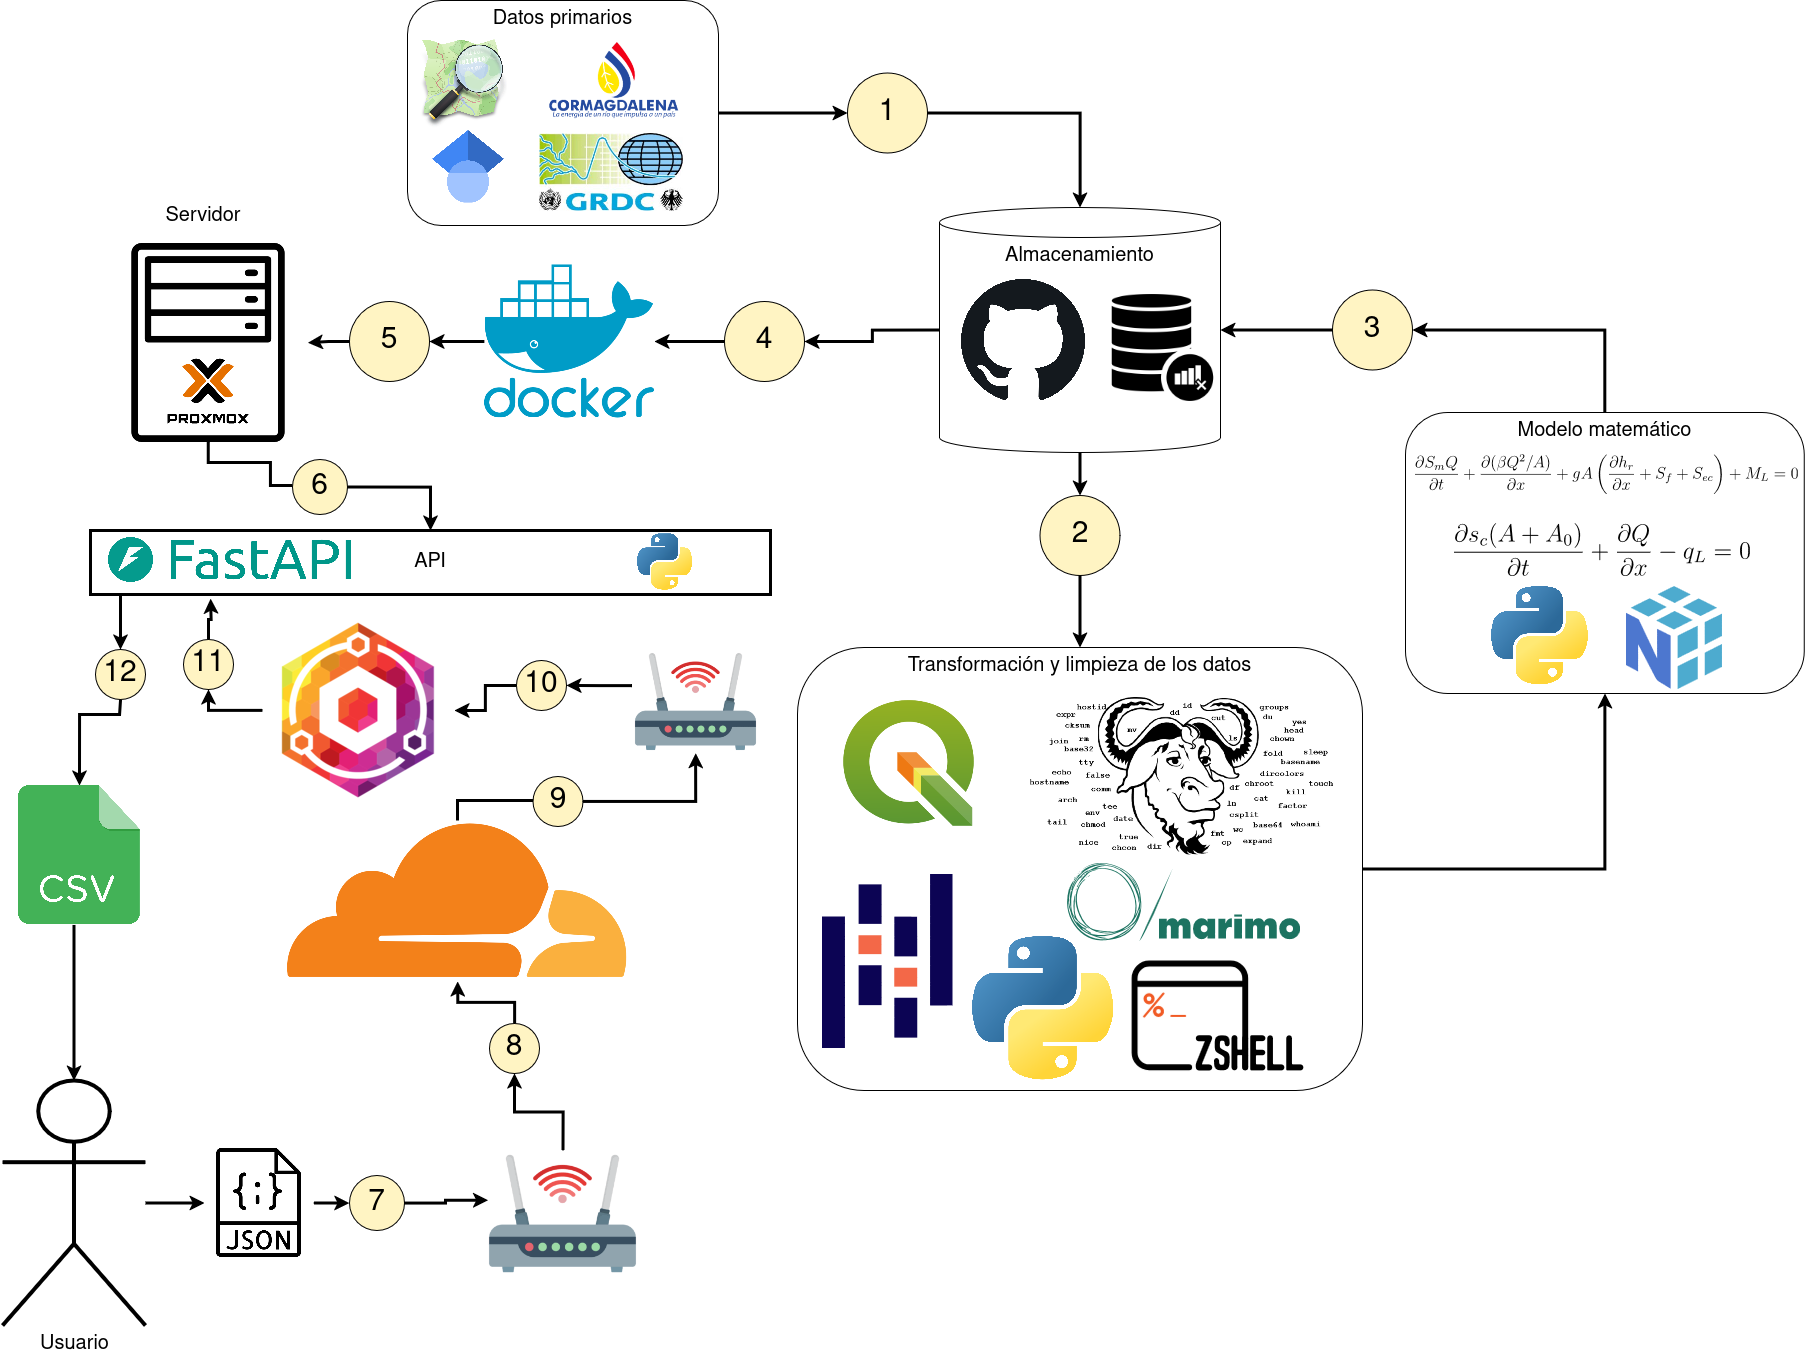
\includegraphics[width=0.9\linewidth]{logos/Arquitectura.png}
     \caption{Arquitectura del funcionamiento y uso de la API.}
     \label{Arquitectura}
   \end{figure}

   
    \begin{figure}[H]
     \centering
     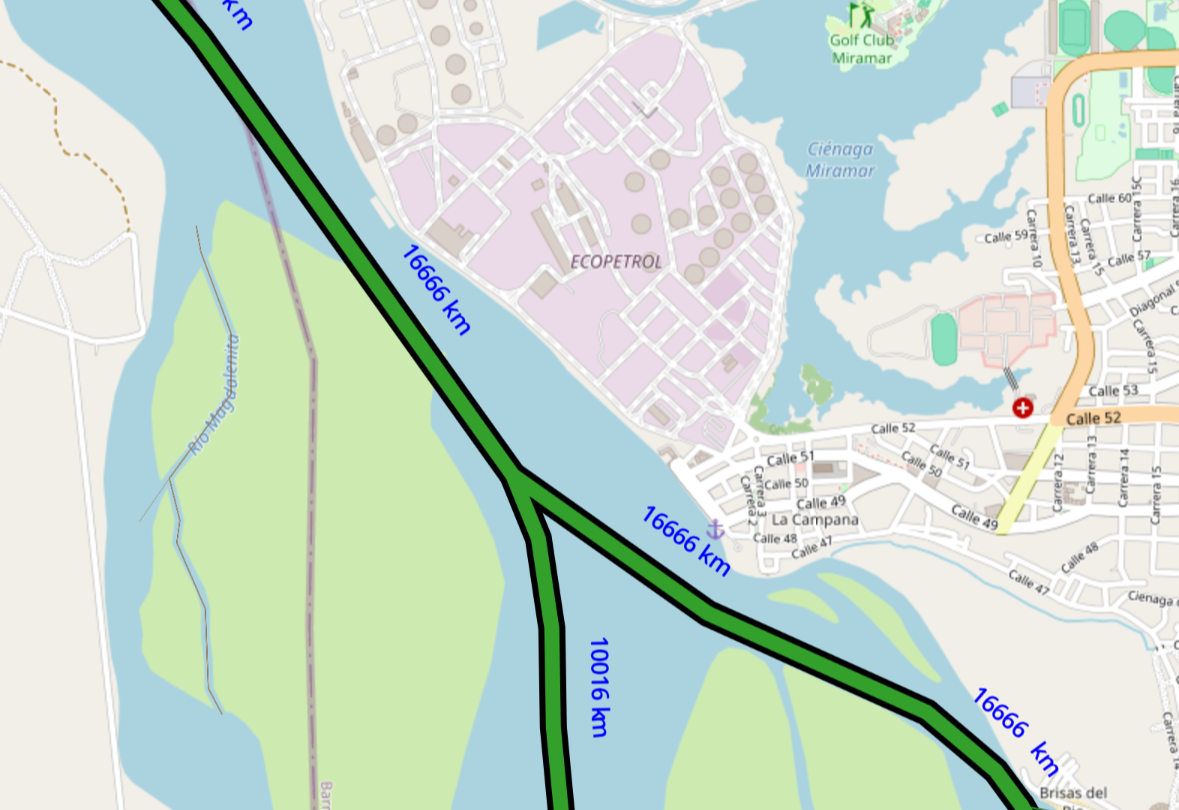
\includegraphics[width=0.8\linewidth]{logos/Waterway.png}
     \caption{Región de estudio para la simulación de demostración, datos de \textit{Waterway}.}
     \label{Region-de-estudio}
   \end{figure}

  \end{alertblock}

  


\end{column}

\separatorcolumn   


\begin{column}{\colwidth}

\begin{block}{RESULTADOS}

   \begin{figure}[H]
     \centering
     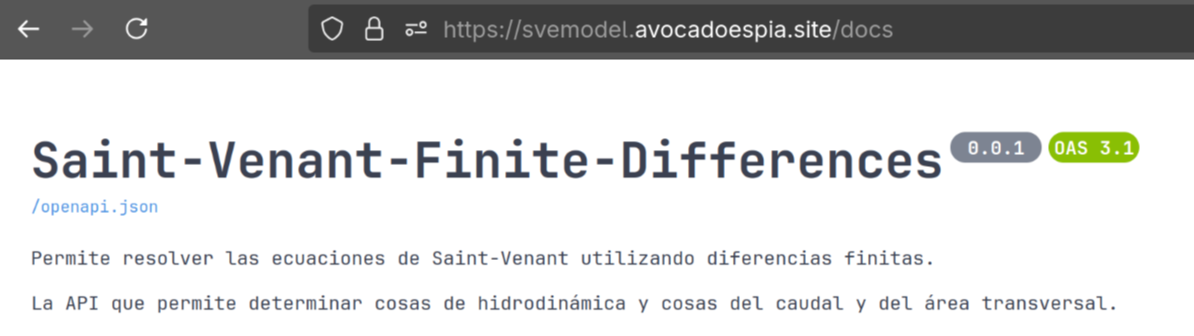
\includegraphics[width=\linewidth]{logos/API1.png}
     \caption{\label{API-1} Documentación de la API ya desplegada en internet bajo el dominio \url{https://svemodel.avocadoespia.site/docs}}
   \end{figure}



   \begin{figure}[H]
     \centering
     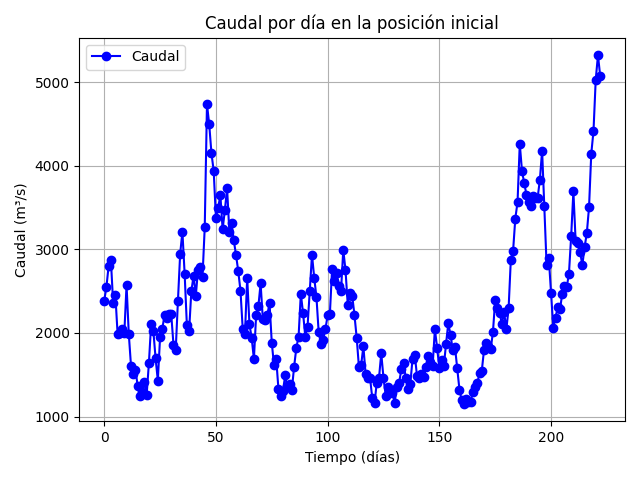
\includegraphics[width=0.7\linewidth]{logos/discharge_upstream.png}
     \caption{Caudal en la posición $x=0$ del Río Magdalena sobre el nivel de Barrancabermeja.}
     \label{API-3}
   \end{figure}     

  \end{block}

  \begin{block}{CONCLUSIONES}

    \begin{itemize}
      \item Se realizó un modelo matemático para aproximar una solución a las ecuaciones de Saint-Venant de continuidad y momentum, utilizando el método numérico de diferencias finitas.
      \item Este trabajo implementó el modelo en el caso del Río Magdalena a la altura de Barrancabermeja, haciendo un trabajo de extracción, limpieza, análisis y modelamiento de datos.
      \item El autor desarrolló e implementó una arquitectura completa de tecnología para estimar el caudal y el área transversal de un río.
    \end{itemize}

  \end{block}

  \begin{block}{REFERENCIAS BIBLIOGRAFÍCAS}

    \begin{thebibliography}{99}

\bibitem{deaton1999dynamic}
Deaton, M., \& Winebrake, J. J. (1999). *Dynamic modeling of environmental systems*. Springer Science \& Business Media.

\bibitem{garcia2020mathematical}
García Rodríguez, F., \& González Carreño, J. O. (2020). *A mathematical model for the simulation of the Magdalena River in the city of Barrancabermeja, Colombia*. Universidad Francisco de Paula Santander. Disponible en: \url{https://repositorio.ufps.edu.co/handle/ufps/1120}. Accedido el 30 de marzo de 2025.
\end{thebibliography}


  \end{block}

    \begin{block}{Agradecimientos}

    Al profesor Javier Riascos por brindar un acompañamiento constante durante la realización del proyecto. A la comunidad de software libre, ya que sin esta no sería posible nada. A mi novia, por brindarme inspiración para la idea del proyecto.

  \end{block}

\end{column}
\separatorcolumn



\end{columns}
\end{frame}

\end{document}
